%% Standalone figure for the Statistical Mechanics exercises (Quiz 1).
%% Build: pdflatex quiz1_sol_compound.tex  (or run build.sh in this folder)
\documentclass[11pt,tikz,border=2pt]{standalone}
\usepackage{amsmath,amssymb}
\usetikzlibrary{arrows.meta, positioning}
\begin{document}
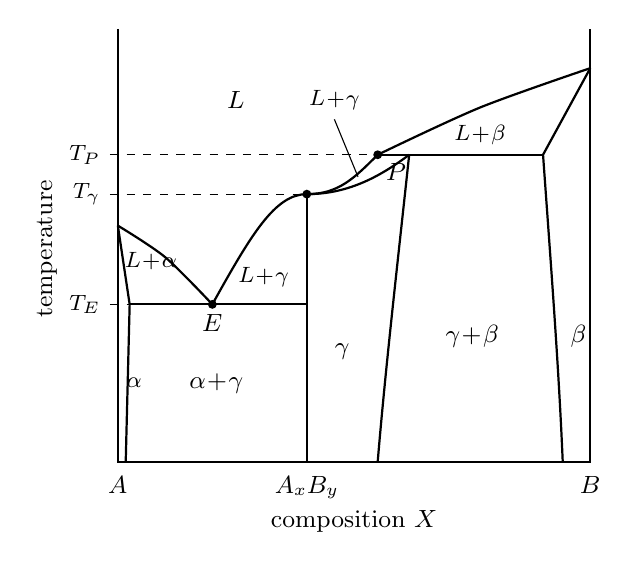
\begin{tikzpicture}[font=\small, >=Latex, line width=0.8pt]
    % frame: A (X=0), compound A_xB_y (gamma, at x=2.4), B (X=1); width 6 cm
    \draw (0,5.5) -- (0,0) -- (6,0) -- (6,5.5);
    % liquidus: A -> E (eutectic) -> congruent point (horizontal tangent) -> P -> B
    \draw plot[smooth] coordinates {(0,3.0) (0.6,2.6) (1.2,2.0)};
    \draw (1.2,2.0) .. controls (1.7,2.9) and (2.0,3.4) .. (2.4,3.4)
                    .. controls (2.8,3.4) and (3.0,3.6) .. (3.3,3.9);
    \draw plot[smooth] coordinates {(3.3,3.9) (4.6,4.5) (6,5.0)};
    % alpha: solidus and solvus
    \draw (0,3.0) -- (0.15,2.0);
    \draw (0.15,2.0) -- (0.10,0);
    % gamma: vertical boundary at the stoichiometric composition, solidus, solvus
    \draw (2.4,0) -- (2.4,3.4);
    \draw (2.4,3.4) .. controls (2.9,3.4) and (3.3,3.6) .. (3.7,3.9);
    \draw (3.7,3.9) .. controls (3.55,2.5) and (3.4,1.2) .. (3.3,0);
    % beta: solidus and solvus
    \draw (5.4,3.9) -- (6,5.0);
    \draw (5.4,3.9) .. controls (5.5,2.5) and (5.6,1.2) .. (5.65,0);
    % three-phase isotherms
    \draw (0.15,2.0) -- (2.4,2.0);
    \draw (3.3,3.9) -- (5.4,3.9);
    \fill (1.2,2.0) circle (1.6pt) node[below] {$E$};
    \fill (3.3,3.9) circle (1.6pt) node[below right=-1pt] {$P$};
    \fill (2.4,3.4) circle (1.6pt);
    % temperature marks
    \begin{scope}[font=\footnotesize]
        \draw[dashed, line width=0.4pt] (-0.1,2.0) node[left] {$T_E$} -- (0.15,2.0);
        \draw[dashed, line width=0.4pt] (-0.1,3.4) node[left] {$T_\gamma$} -- (2.4,3.4);
        \draw[dashed, line width=0.4pt] (-0.1,3.9) node[left] {$T_P$} -- (3.3,3.9);
    \end{scope}
    % region labels
    \node at (1.5,4.6) {$L$};
    \node[font=\footnotesize] at (0.42,2.55) {$L\!+\!\alpha$};
    \node[font=\footnotesize] at (1.85,2.35) {$L\!+\!\gamma$};
    \node[font=\footnotesize] at (4.6,4.15) {$L\!+\!\beta$};
    \node at (1.25,1.0) {$\alpha\!+\!\gamma$};
    \node at (2.85,1.4) {$\gamma$};
    \node at (4.5,1.6) {$\gamma\!+\!\beta$};
    \node at (5.85,1.6) {$\beta$};
    \node[font=\footnotesize, right=-2pt] at (0.05,1.0) {$\alpha$};
    \draw[line width=0.4pt] (3.05,3.62) -- (2.75,4.35) node[above, font=\footnotesize] {$L\!+\!\gamma$};
    % axes
    \node[below] at (0,-0.05) {$A$};
    \node[below] at (2.4,-0.05) {$A_xB_y$};
    \node[below] at (6,-0.05) {$B$};
    \node[below=14pt] at (3,0) {composition $X$};
    \node[rotate=90] at (-0.9,2.7) {temperature};
\end{tikzpicture}
\end{document}
